\documentclass[11pt]{article}
\usepackage{graphicx}
\usepackage{listings}
\usepackage{multirow}
\usepackage{color}
\usepackage[english]{babel}
\usepackage{placeins}
 \usepackage{url}
 \usepackage{mathtools}
\usepackage{enumerate}
%\usepackage{mylingmacros}

\begin{document}
\newcommand\add[1]{{\textcolor{blue}{ADD: #1}}}
\newcommand\modi[1]{{\textcolor{green}{MODIFIED: #1}}}
\newcommand\remove[1]{{\textcolor{red}{REMOVE: #1}}}
\newcommand\expand[1]{{\textcolor{blue}{EXPAND: #1}}}
\newcommand\rewrite[1]{{\textcolor{green}{REWRITE: #1}}}

% Titre complet


\title{Data expansion for semantic classification}

\author{Anna Liednikova\\
Supervisor: Claire Gardent}




\maketitle

\tableofcontents

\clearpage

\section{Introduction}
\label{sec:}
 
This project was set within the framework of a collaboration with the
ALIAE startup whose aim is to develop a chatbot to collect
information from clinical patients. The main idea is to replace
strictly defined surveys by a more natural conversation in order to
let users express themselves freely so that more information could be
collected.

The chatbot consists of two main modules:
\begin{itemize}
\item NLU (Natural Language Understanding): interpreting the user input
\item Dialog Managment: deciding how to respond to the user input and
  generating the system response
\end{itemize}


\begin{figure}[htbp]
\begin{center}
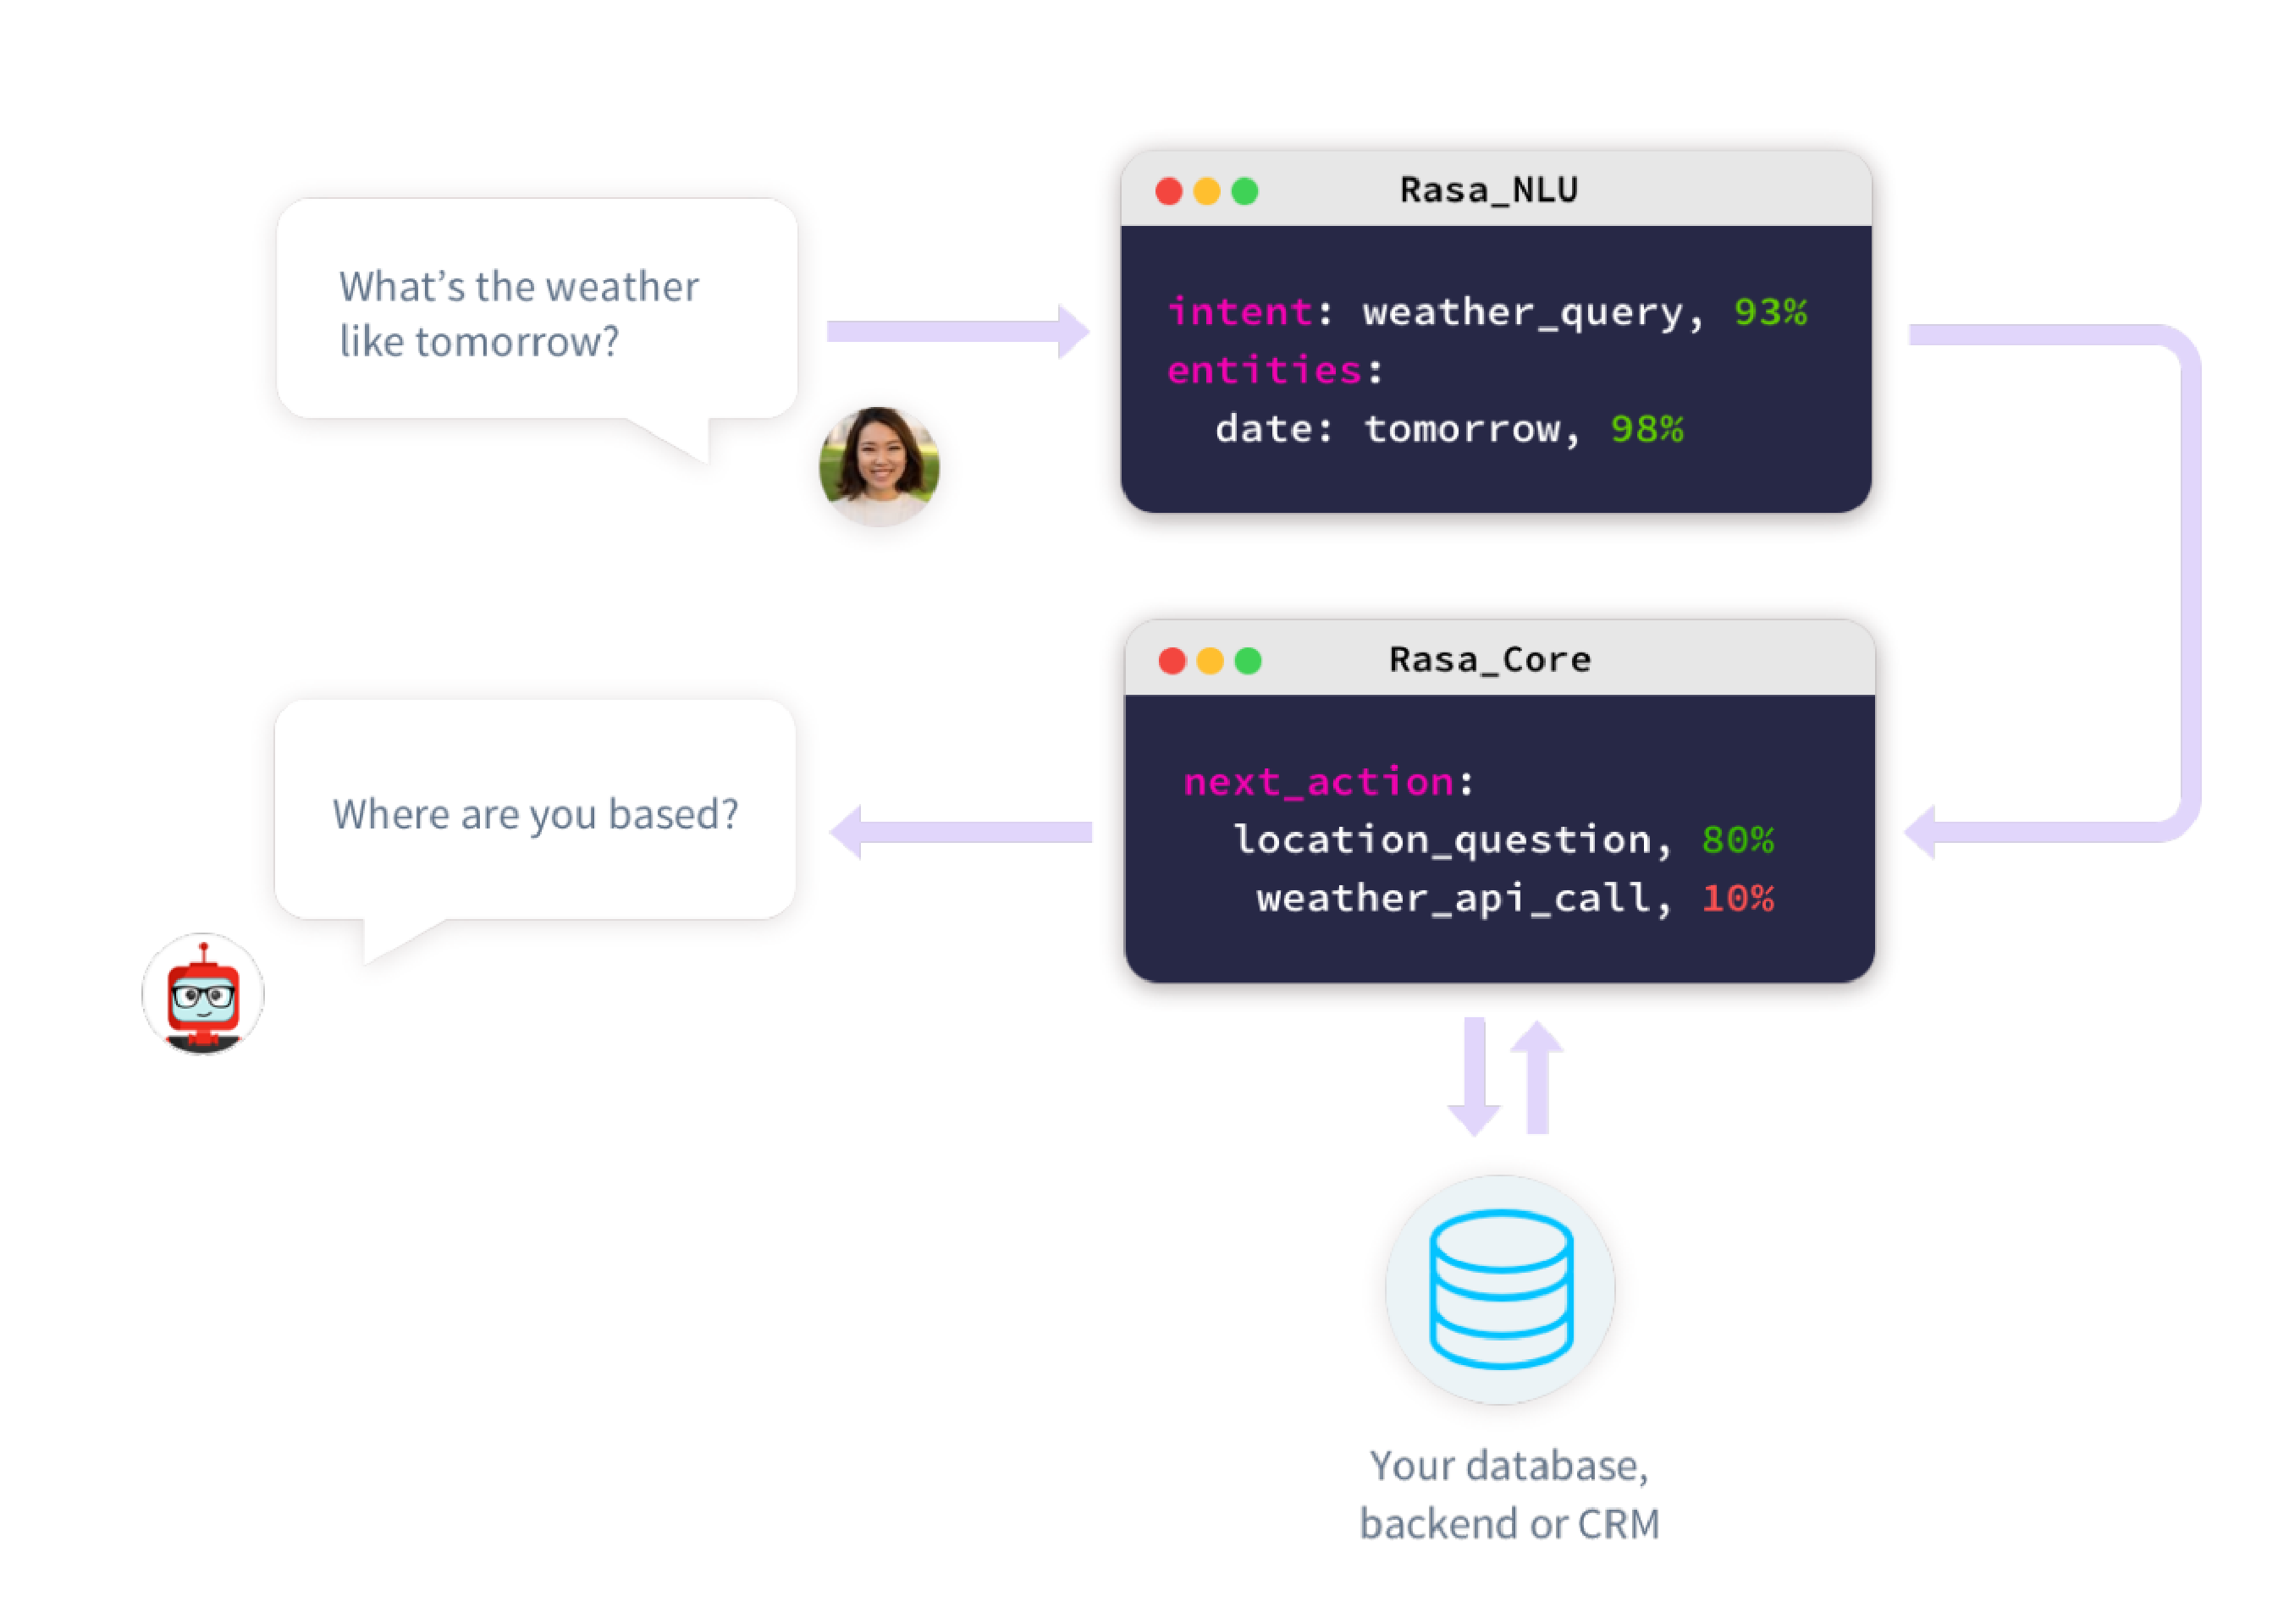
\includegraphics[width=.9\textwidth]{img/rasa.pdf}
\end{center}
\caption{}
\label{fig:rasa}
\end{figure}
In this project, we focus on natural language understanding and
consider a simplified notion of understanding where each user input is
mapped to an ``intent''. Given a pre-defined and finite set of intents
(Does the user speaks about pain, physical activity etc. ?), the aim
of the NLU module is to assign each user input an intent\footnote{We
  make the simplifying (and incorrect) assuption that the user input
  contains a single intent.}. The detected intent is then used, in
conjunction with additional information extracted from the previous
dialog interactions, to determine how to
respond (cf. Figure~\ref{fig:rasa}\footnote{The figure
  actually shows a more complex notion of understanding where the user
  utterance is mapped not only to an intent but also to a set of
  entities. In this work, we focus on how to improve intent detection
  and leave entity detection for future research.}).

\section{Goals and Methodology}
\label{sec:goals}


The NLU module is a classifier which given a user input, predicts the
corresponding intent. Our goal is to improve this classifier starting
from a small training set (roughly 100 utterance/intent pair for each
intent) and automatically expanding this labelled data. To this
end, we developed a semi-supervised data expansion technique which
permits expanding the initial data with utterances extracted from a
medical forum. We show that the expanded data permits improving the
classifier by \add{ADD NB of improvment points} accuracty points.

This report is structured as follows. Section~\ref{sec:relatedwork}
briefly reviews the state of the art and situates our proposal with
respect to related work.  Section~\ref{sec:methodology} presents the
methodology used for data expansion. Section~\ref{sec:datasets} describes
the datasets used. Section~\ref{sec:xps} reports on the experimental
setting and on the results. Section~\ref{sec:conclusion} concludes
with pointers for further research.

\section{Literature review}
\label{sec:relatedwork}

\cite{N18-2058} \modi{present an approach for automatically generating additional training data for event extraction systems}. First, they trained a baseline classifier on available data. Then, they cluster external data to obtain cluster of paraphrases using the NewsSpike method introduced by \cite{zhang2015}. They then label the clusters using the baseline model trained on the initial dataset of labelled data. Combining the new labelled data and the original one, they then retrained the event extractor.

\section{Methodology}
\label{sec:methodology}

Our methodology for data expansion falls into two main steps. First, we compare different methods for representing utterances using both clustering and classification (Sections~\ref{subsec:sentencerepresentations} and ~\ref{subsec:clustering}). Second, based on the best sentence representations, we gradually increment the size of the labelled data and iteratively train new classifiers on the extended data (Section~\ref{subsec:dataexpansion}). 

%% We follow \cite{N18-2058} methodology. Instead of using \cite{zhang2015}'s methods for identifying clusters of related sentences however, we explore different ways of representing sentences using deep learning approaches. We then apply clustering to the resulting sentence representations. Finally, we investigate the impact of the extended labeled data on classification. 

%% irst
% group together paraphrases of event mentions.

%% then use the simple examples in each cluster to as-
% sign a label to the entire cluster

%% com-
% bine the new examples with the original training
% set and retrain


\subsection{Building Sentence Representations}
\label{subsec:sentencerepresentations}
We explore two ways of building sentence representations: Word2vec and LDA. %% he good point of using these models is that they can be used for both word and sentence representation since one word can be treated as a small sentence. That can help us also to create sentence representations in two steps using machine and deep learning techniques. First, we map words to continuous representations. Second, we combine these word representations into sentence representations using BiLSTM encoder. \add{bibref}.

%We construct sentence representations out of the word representations described in the previous section using two types of neural networks:  PositionwiseFeedForward \cite{vaswani2017attention} and BiLSTM \add{bibref}.

\paragraph{LDA.}

One of the most common methods for constructing thematic models is the Latent Dirichlet Allocation (LDA) $\cite{lda_def}$ that models a document as a distribution of topics and a topic as a distribution of words. Here a document is a sentence. Hence a sentence is represented as a distribution of topics. 

\add{an example of topics produced by an LDA model}
\begin{lstlisting}
[(0.13819554, 'sleep'),
  (0.10817484, 'morning'),
  (0.10187448, 'sometimes'),
  (0.09861754, 'help'),
  (0.060275868, 'able'),
  (0.060111083, 'nap'),
...],
\end{lstlisting}


And here is an example representation for a  sentence/ 

\add{an example of document representation as a distribution over topics}

%If we want represent just one word we can just treat it like a small sentence and have the same output.

The LDA algorithm is based on the Dirichlet prior distribution and
assumes a bag-of-words model - a model for analyzing texts
that takes into account only the frequency of words, but not their
order. This model is well suited for thematic modeling, since it
permits detecting implicit relationships between words. The LDA
method performs soft clustering and assumes that each word in the
sentence is generated by some latent topic, which is determined by a
probability distribution on the set of all words of the text.


\paragraph{Word2Vec.} Word2Vec representations are low dimensional vectors also called embeddings which are built based on textual
cooccurences and learned using shallow, two-layer neural networks
\cite{Mikolov2013EfficientEO}. Given a large corpus of text as input,
Word2Vec produces a vector space where words that share common
contexts in the input corpus will be mapped to vectors that are close
to one another in the vector space.

%x$https://papers.nips.cc/paper/5021-distributed-representations-of-words-and-phrases-and-their-compositionality.pdf$

To build sentence representations, we simply average the Word2Vec
vectors of the content words present in that sentence.

%% \paragraph{Bi-LSTM.} The general idea of BiLSTM layer is repeating the first recurrent layer in the network so that they are next to each other and then providing the straigh input sequence as input to the first level and an inverse copy of it for the second.

%% In more formal way, for the sequence of words $T \{w_{t}\}_{t = 1, ..., T}$ bidirectional LSTM computes a set of T vectors $\{h_{t}\}_{t}$. For $t ∈ [1 ,. ,,, T]$, $h_{t}$ is the combination of forward and backward LSTM, that read sentences in two opposite directions. 

%% We experiment with two ways of combining a changing number $(h_{1}, ..., h_{T})$ to form a vector of a fixed size, either by choosing the last hidden state $h_{T}$ (BiLSTM-last), or either by selecting the maximum value over each dimension of the hidden units (max pooling) (Collobert and Weston, 2008) or by considering the average of the representations (mean pooling). The choice of these models is motivated by their demonstrated effectiveness in embedding models (Conneau et al., 2018) 


\subsection{Clustering Sentences}
\label{subsec:clustering}
Using the sentence representations described in the previous section,
we apply clustering to group together sentences that are similar.  We
set the number of clusters to the number of intents (20) and we use
not only purity and Silhouette coefficients to evaluate the clusters
but also homogeneity and completeness to better assess how the
resulting clusters correlate with initial intents. Also, for each
model, we plot a confusion matrix with a background gradient to
visualize how well clusters separate different intents. Based on these
metrics and vizualisation, we determine which method produces
representations that best support intent detection.

We compare three clustering algorithms:

\begin{itemize}
\item K-Means (KM)
\item Agglomerative Clustering (AG)
\item Gaussian Mixture (GM)
\end{itemize}


\paragraph{K-Means.} The basic idea is to define K centroides one for each cluster. It is best to place them as far apart as possible. The next step will be to accept each point belonging to this data set and associate it with the precision of the centroid. If no point is under consideration, the first stage is completed. At the moment, we need to re-calculate K's new centroids, as the cluster barycenter that stems from the previous step. After these new centroids appear on us, a new binding must be made between the same points of the data set and the nearest new center of gravity. A loop is created. As a result of this cycle, we can see that k centroids change their location step by step until any changes are made. In other words, centroids are no longer moving.

The algorithm is aimed at minimizing the target function, in this case, the quadratic error function. Target function:
\begin{equation}
J = \sum_{j=1}^{k} \sum_{i=1}^{n} (\Vert x_{i}^{(j)} - c_{j} \Vert)^{2}
\end{equation}

where $(\Vert x_{i}^{(j)} - c_{j} \Vert)^{2}$ is the chosen distance between the data point $x_{i}^{(j)}$ and center $c_{j}$, it is an indicator of the distance n of the data points from their respective cluster centers.

Centroid is defined as follows:

\begin{equation}
c_{j} = \dfrac{1}{N} \sum_{i=1}^{N} x_{i}^{(j)}
\end{equation}

where $x_{i}^{(j)}$ is the point belonging to the cluster $J$, $N$ - total number of points in the cluster.

\paragraph{Agglomerative Clustering} is a kind of hierarchical clustering with 'bottom-up' approach when new clusters are created by combining smaller clusters and, thus, a tree is created from leaves to trunk \cite{ward63:_hierar_group_optim_objec_funct}. The main feature of the agglomerative hierarchical clustering method is that if we want to get a different number of clusters, we will not need to restart the algorithm, because the whole tree is calculated, and then we say that we want to cut it in some place.


Different linkage criterions can be used to calculate distance between sets of observation. Ward’s method minimizes the variance of the clusters being merged. This method is used for tasks with closely spaced clusters. The euclidian distance between clusters is taken as the increment of the sum of squares of the distances of objects to the center of the cluster, obtained as a result of their combination: 

\begin{equation}
\Delta = \sum_{i} {(x_{i} - {\bar {x}})^{2}} - \sum_{x_{i} \in A} (x_{i} - {\bar {a}})^{2} - \sum_{x_{i} \in B} (x_{i} - {\bar {b}})^{2}
\end{equation}

At each step of the algorithm, these two clusters are combined, which lead to a minimal increase in variance.



\paragraph{Gaussian Mixture.}

\rewrite{In statistics, a mixture model is a probabilistic model for representing the presence of subpopulations within an overall population, without requiring that an observed data set should identify the sub-population to which an individual observation belongs. Formally a mixture model corresponds to the mixture distribution that represents the probability distribution of observations in the overall population without sub-population identity information.}

A Gaussian mixture model \cite{reynolds2015gaussian} represents a weighted sum of M Gaussian densities elements for D-dimensional continuous-valued data vectors:

\begin{equation}
p(x|\lambda) = \sum_{i=1}^{M} w_{i} g(x|\mu_{i}, \sum_{i})
\end{equation}

where each Gaussian densities element defined as 

\begin{equation}
g(x|\mu_{i}, \sum_{i})=\frac{1}{(2\pi)^{\frac{D}{2}}|\sum_{i}|^{\frac{1}{2}}} e^{-\frac{1}{2}(x-\mu_{i})'\sum_{i}(x-\mu_{i})} 
\end{equation}

with mean vector $\mu_{i}$ and covariance matrix $\sum_{i}$. The mixture weights satisfy the constraint that $\sum_{i=1}^{M} w_{i} = 1$.

GMM parameters are estimated from training data using the iterative Expectation-Maximization (EM) algorithm or Maximum A Posteriori (MAP) estimation from a well-trained prior model.

%$https://pdfs.semanticscholar.org/734b/07b53c23f74a3b004d7fe341ae4fce462fc6.pdf$


\subsection{Semi-Supervised approach to Data Expansion and Classification}
\label{subsec:dataexpansion}

After choosing the best model for representing sentences, we
iteratively expand the training data and train the corresponding
classifiers as follows.


\begin{itemize}
\item \textbf{Step 1: Classification.} Apply the classifier trained on the currently available labelled data to a set of unlabelled sentences;
\item \textbf{Step 2: Clustering.} Clusterize these unlabelled sentences into 200 clusters
\item \textbf{Step 3: Filtering.} Use the probability and the label assigned by the classifier to each unlabelled sentence to :
  \begin{itemize}
\item Eliminate sentences whose probability is below a given threshold
\item Eliminate clusters with less than $m$ members
  \end{itemize}
\item \textbf{Step 4: Data expansion.} Add to training data the $n$ best labelled items for each intent. 
  \item \textbf{Step 5: Classifier Training.} Train a new classifier using both the previous and the new labelled data. 
\end{itemize}

\paragraph{Classification.} For classification, we use SVC (Support Vector Classifier). The main idea of ​​the method is transfering the initial vectors into a space of higher dimension and searching for a separating hyperplane with the maximum gap in this space. Two parallel hyperplanes are built on both sides of the hyperplane separating the classes. The separating hyperplane will be the one that maximizes the distance to two parallel hyperplanes. The algorithm works under the assumption that the greater the difference or the distance between these parallel hyperplanes, the less will be the average classifier error.  Due to the small size for dataset it's essential to create balanced training and test datasets.

The initial labelled dataset was provided by ALIAE (gold data). We split our gold dataset into train and test sets and systematically use the test set for evaluation and comparison of the classifiers learned on the different datasets produced during data expansion.

At each iteration during data expansion, we use the classifier trained
on the data created at the previous iteration to label unlabelled
sentences extracted from some external source. 

\paragraph{Clustering.} To expand the training data, we retrieve utterances from a medical forum. The unlabelled data is then built based on these utterances after some filtering is applied to eliminate sentences that are either out of topic or too complex (cf. Section~\ref{sec:}). Next we build representations for these unlabelled sentences using the techniques described in Section~\ref{sec:} and we apply clustering to create 200 clusters. 

\paragraph{Filtering.} The SVC classifier assigns each unlabelled sentence a category (an intent) and a probability. We eliminate from the clusters all those sentences whose probability is below a given threshold. We then eliminate all clusters whose size is less than a set minimum. 

For our subset we find the best clusterization by elbow method \cite{elbow_rule}. Later, having both labels for intent and cluster, we leave just that clusters that populated by items with maximum probability that allows us to cover all intent with new examples.

For each cluster we calculate number of intent representators and their overall distribution. We then keep only those clusters where some intent is represented more than in average. Elements of clusters that are left will be labelled by the majority.


\paragraph{Data Expansion.} Finally, we select N labelled items for each category/intent and extend the training data with them to update sentence representation and classification models.

We repeat this cycle until we won't be able to extend train dataset by additional samples or classifier score will stop to grow.

\section{Datasets}
\label{sec:datasets}

For our task we have two dataset. The first one is labelled by human and the second one was retrieved from the web to extend the previous one. Our goal was to use web data to expand the training set and improve the classifier which assigns each sentence an intent. 

\subsection{Labelled Data}
\label{subsec:labelleddata}
The initial dataset was created manually by the Aliae startup and  covers 20 main possible users intents. Each sentence represents one intent e.g., 
%\enumsentence{
\begin{description}
\item[Text:] After sleep, for 2-3 hours, I am better and then start feeling tired again
\item[Intent:] sleep
\end{description}
%}

The distribution of labels is shown in Figure~\ref{figure:name}. There
are in average, 3.4 words per sentence (min: 0, max: 12, std:
2.16367).  The total number of sentences is 3305 and the vocabulary
consists of 1882 content words (after removing stopwords).

 \begin{figure}[h]
 	\centering
 	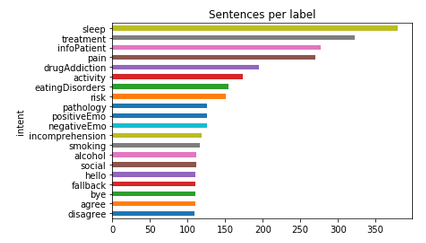
\includegraphics[scale=0.4]{report1.png}
	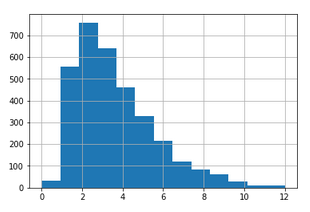
\includegraphics[scale=0.45]{report4.png}	
	\caption{Left: Label distribution in dataset, Right: Distribution of sentence length}
 \label{figure:name}
 \end{figure}
\FloatBarrier


\subsection{Forum data}
\label{subsec:forumdata}

To improve the initial classifier, we needed to extend the training
dataset by much more data and more naturally constracted one. Looking
for open medical dataset that can be used for this purpose, we found
\cite{zhang2015} and \cite{sondhi-EtAl:2010:POSTERS} works that used
the HealthBoards forum data for similar tasks. 
HealthBoards\footnote{\url{healthboards.com}} is a medical forum web portal that
allows patients to discuss their ailments.


We scraped 272553 unique posts labelled with 238 forum
categories. Figure~\ref{forum_data_stat} shows the dataset
statistics. In average, sentences contain $11\pm7$ words after
preprocessing.


 \begin{figure}[h]
 	\centering
 	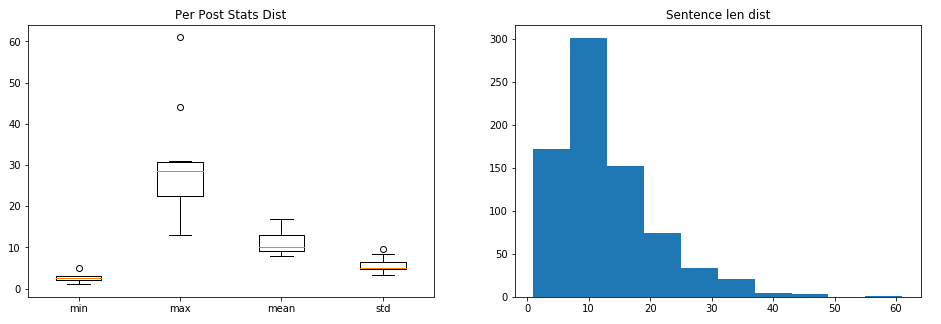
\includegraphics[scale=0.4]{report3.png}
	\caption{Text stat}\label{forum_data_stat}
 \end{figure}
\FloatBarrier

This dataset has precise categorization so that some posts are more specialized and some are out of the scope of our intent labels. We should start with the data that is most similar to the initial one, so that's why we choose categories of boards that are similar to our intents. This will help us to be able gradually expand the existing context. So we will keep posts of categories provided in table \ref{cat_freq}.


%\add{scrape posts; select categories that are relevant (listed in Table \ref{cat_freq}); keep only these post that have the relevant categories + length constraints}

\begin{table}[htb]
\centering
\begin{tabular}{ |r|c| }
\hline
Category of board &  \# of posts \\ \hline
digestive-disorders & 5064 \\ \hline
addiction-recovery & 3644 \\ \hline
sleep-disorders & 1748 \\ \hline
smoking-cessation & 937 \\ \hline
eating-disorder-recovery & 762 \\ \hline
chronic-pain & 735 \\ \hline
chronic-fatigue & 662 \\ \hline
stress & 415 \\ \hline
family-friends-addicts-alcoholics & 312 \\ \hline
pain-management & 25 \\ \hline
\end{tabular}
\caption{Selected categories}\label{cat_freq}
\end{table}
\FloatBarrier

Finally, the corpus consists of N  sentences. 

Also, for big number of iterations data should be divided in subsets by increasing sentence length because of the difference in mean values for both datasets. So after tokenizing posts into sentences we calculate it's length. For each iteration, we only leave sentences which have mean+std words after pre-processing (cf. Section~\ref{subsec:preprocessing}).


\section{Experiment}
\label{sec:xps}

Experiment consists of the main stages:

\begin{itemize}
\item preprocess text of labelled and unlabelled data
\item use clustering to choose between different ways of representing sentences
\item training a classifier on the labelled data
\item iterative semi-supervised learning:
  \begin{itemize}
  \item data expansion (cf Section \ref{subsec:dataexpansion}) ; 
  \item update sentence representations (using new data and old parameters)
  \item retrain on classifier on gold + new labelled data
  \item evaluate new classifier on gold test data
\end{itemize}
\end{itemize}

\subsection{Preprocessing routine}
\label{subsec:preprocessing}
The textual data was segmented into sentences, tokenized and lemmatized using NLP
libraries. Stop words were removed.

We compared two libraries, NLTK and SpaCy.

For example, in word tokenization they give different results that can influence not only simple statistics but meaning too. Some example of different tokenization can be seen in table \ref{token_dif}. Though concating words to ones like 'flulike' or '35mg' or 'longterm' sometimes gives more robust and concrete meaning in case of big dataset, in our case it seems better to stay with SpaCy way of tokenization in order to have smaller and more simple vocabualary.

\begin{center}
\begin{table}
\begin{tabular}{ |p{7cm}|p{7cm}| }
\hline
NLTK & SpaCy \\ \hline
['i', 'wouldnt', 'go', 'to', 'sleep', 'until', 'like', '5', '6', 'or', '8am'] & 
['i', 'would', 'nt', 'go', 'to', 'sleep', 'until', 'like', '5', '6', 'or', '8', 'am'] \\ \hline
['that', 'is', 'totally', 'wrongheaded'] & ['that', 'is', 'totally', 'wrong', 'headed'] \\ \hline
['i', 'am', 'in', 'the', 'process', 'of', 'tapering', 'from', 'suboxone', 'longterm', 'use'] & 
['i', 'am', 'in', 'the', 'process', 'of', 'tapering', 'from', 'suboxone', 'long', 'term', 'use'] \\ \hline
['i', 'had', 'an', 'onandoff', 'opiateopioid', 'habit', 'from', 'about', '2010'] & 
['i', 'had', 'an', 'on', 'and', 'off', 'opiate', 'opioid', 'habit', 'from', 'about', '2010'] \\ 
\hline
['i', 'have', 'flulike', 'pathologysymptom'] & ['i', 'have', 'flu', 'like', 'pathologysymptom'] \\ \hline
['i', 'have', 'exerciseinduced', 'insomnia'] & ['i', 'have', 'exercise', 'induced', 'insomnia'] \\ \hline
['i', 'm', 'supposed', 'to', 'take', '6', '35mg', 'tablets', 'a', 'day', 'but', 'i', 'have', 'taken', '20', 'today'] & 
['i', 'm', 'supposed', 'to', 'take', '6', '35', 'mg', 'tablets', 'a', 'day', 'but', 'i', 'have', 'taken', '20', 'today'] \\ 
\hline
\end{tabular}	
\caption{Tokenization comparison}\label{token_dif}
\end{table}
\end{center}
\FloatBarrier

For stopwords removing there were three options: nltk, spacy and the longest one. The last option was rejected due to containing words like 'want', 'stop', 'successfully' etc. that can be useful for detecting basic intents like positive or negative emotion, social. Finally nltk one was selecting because of containing shorts like 'm' from 'am', 've' from 'have'. Final dictionary contained 1882 words. Also all numbers were changed to num. Chart (\ref{words_freq}) looks fine.

 \begin{figure}[h]
 	\centering
 	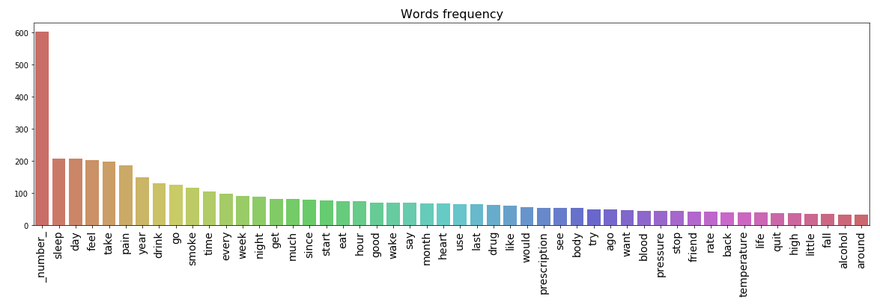
\includegraphics[scale=0.4]{report2.png}
	\caption{Words frequency}
 \label{words_freq}
 \end{figure}
\FloatBarrier

Next problem we faced is empty sentences. But there is not a lot of occurances, so their dropping don't change the dataset much.

\begin{tabular}{ |r|l| }
\hline
intent & items \\ \hline
fallback          & 12 \\ \hline
disagree          & 11 \\ \hline
hello             &  4 \\ \hline
agree             &  3 \\ \hline
incomprehension   &  2 \\ \hline
positiveEmo       &  1 \\ \hline
\end{tabular}

These sentences are: 'what?', 'same that again', 'I am up', 'same', 'can you',
       'do that', 'do this', 'Will do', 'no', 'no i will not',
       "No i don't", 'no', 'no i will not', "No i don't", "What's up?",
       "What's up?", 'he', 'a', 'd', 'i', 'm', 'o', 's', 't', 'y',
       'I will', 'Will do', 'No', 'no', 'No it is not', "No I don't",
       'No', "I'm here"


\subsection{Clustering for sentence representation evaluation}
\label{subsec:clustering2}
\add{used to compare different ways of representing sentences}

Forum data is splitted into 20 (number of intents) cluster to be able to see how current representation can reflect desirable labels. Also, it can provide us with information which classes will be easier to identify and which can mix with others.


For selecting the best model we changed space dimension (topics for LDA and features for W2W). Preferred number of features for W2V model is 200. It's the start point for our model.

\subsubsection{Evaluation metrics}

For every model following metrics and their average were calculated: purity score, Silhouette Coefficient, homogeneity and completeness scores. Later for each parameter average among clustering models calculated for each score in order to get both table and plot.

Also for each model confusion matrix created between cluster labels and initial intents.

\paragraph{Purity} is calculated by assigning each cluster to the class that is most often found in the cluster, and then the accuracy of this assignment is measured by counting the number of correctly assigned documents and dividing by N.

\begin{equation}
\centering
purity(\Omega,C) =\frac{1}{N} \sum_{k} \max_{j}|\omega_{k}\cap c_{j}|
\end{equation}
where $\Omega=\{\omega_{1}, \omega_{2}, ... ,\omega_{K}\}$ is the set of clusters and $C = \{c_{1}, c_{2}, ... , c_{J}\}$ is the set of classes. 

\paragraph{Silhouette Coefficient} shows how much the average distance to objects of its cluster differs from the average distance to objects of other clusters. This value is in the range $\lfloor 0, 1\rfloor$. Values close to -1 correspond to poor (scattered) clustering, values close to zero indicate that the clusters intersect and overlap each other, values close to 1 correspond to "dense" clearly selected clusters. Thus, the larger the silhouette, the more clearly highlighted the clusters, and they are compact, tightly grouped clouds of points.

\paragraph{Homogeneity and completeness.} Homogeneity will be maximal if the cluster consists only of objects of one class. Completeness will be maximum if all objects from the class belong to only one specific cluster.
Formally, these measures are also determined using the functions of entropy and conditional entropy, considering the partitioning of the sample as discrete distributions:

\begin{equation}
h = 1 - \frac{H(C|K)}{H(C)}, c = 1 - \frac{H(K|C)}{H(K)}
\end{equation}

here is $K$ the result of clustering, is $C$ the true partitioning of the sample into classes. Thus, $h$ measures how much each cluster consists of objects of one class, and $c$ measues how much objects of one class belong to one cluster.
\subsubsection{Word2Vec model}

We compare results for different embedding size ranging from 10 to 600.

\begin{center}
\begin{tabular}{ |c|c|c|c|c|c| }
\hline
Embedding Dim.  & purity  & silhouette  & homogeneity  & completeness\\ \hline 
10  & 0.183157  & 0.0680834  & 0.108901  & 0.12661\\ \hline 
20  & 0.182854  & 0.0506986  & 0.111099  & 0.124805\\ \hline 
30  & \textbf{0.185477}  & 0.0683824  & 0.110799  & 0.132563\\ \hline 
50  & 0.184569  & 0.0647393  & \textbf{0.111876}  & 0.131964\\ \hline 
100  & 0.182148  & \textbf{0.0813837}  & 0.108022  & 0.138329\\ \hline 
150  & 0.183661  & 0.0298524  & 0.106401  & 0.141179\\ \hline 
200  & 0.176803  & 0.0581627  & 0.103708  & 0.141973\\ \hline 
300  & 0.176097  & 0.0432732  & 0.106379  & 0.151118\\ \hline 
400  & 0.169642  & 0.0626822  & 0.100455  & 0.148768\\ \hline 
500  & 0.168533  & 0.0653733  & 0.0976706  & 0.146799\\ \hline 
550  & 0.17176  & 0.0584935  & 0.0994422  & \textbf{0.151185}\\ \hline 
600  & 0.169138  & 0.0574187  & 0.0980455  & 0.150695\\ \hline \end{tabular}
\end{center}
\FloatBarrier

\begin{figure}[h]
\centering
 	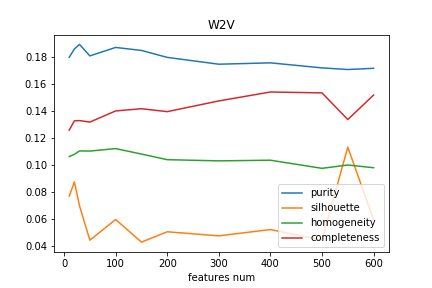
\includegraphics[scale=0.7]{w2v_scores.png}
	\caption{LDA scores}
\label{w2v_scores}
\end{figure}
\FloatBarrier

Later we will try both 10 and 100 features.

\begin{figure}[h]
	\centering
 	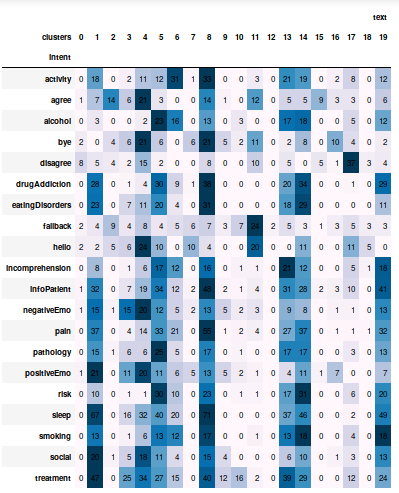
\includegraphics[scale=0.7]{best_w2v_cm.png}
	\caption{W2V confusion matrix}
 \label{w2v_cm_mat}
 \end{figure}
\FloatBarrier

\subsubsection{LDA model}

We iterated through different numbers of topics for LDA model to see which one should be used to represent our dataset. In table \ref{LDA_num_topic} we can see the comparison. 

\begin{table}[htb]
\begin{center}
\begin{tabular}{ |c|c|c|c|c| }
\hline
num & purity  & silhouette  & homogeneity  & completeness \\ \hline 
10  & 0.253656  & 0.461589  & 0.157498  & 0.178928  \\ \hline 
20  & 0.259203  & 0.378276  & 0.168191  & 0.182203  \\ \hline 
30  & 0.251538  & 0.331069  & 0.157755  & 0.168448  \\ \hline 
50  & 0.240545  & 0.287032  & 0.147430  & 0.166824  \\ \hline 
100  & 0.266465  & 0.187596  & 0.168647  & 0.189221 \\ \hline 
150  & 0.256077  & 0.167888  & 0.161589  & 0.185054 \\ \hline 
200  & 0.263843  & 0.149212  & 0.175117  & \textbf{0.194913} \\ \hline 
300  & 0.250025  & 0.151526  & 0.165607  & 0.184314 \\ \hline 
400  & \textbf{0.272718}  & 0.192777  & \textbf{0.177547}  & 0.192270 \\ \hline 
500  & 0.259506  & \textbf{0.203725}  & 0.174925  & 0.192831 \\ \hline 
550  & 0.229450  & 0.166200  & 0.149270  & 0.158548 \\ \hline 
600  & 0.254261  & 0.191729  & 0.171744  & 0.186001 \\
\hline 
\end{tabular}
\caption{Comparision of LDA with different number of topics}
\label{LDA_num_topic}
\end{center}
\end{table}
\FloatBarrier

The best model - is LDA with 400 topics according to scores and with priority to purity and homogeneity ones.

\begin{figure}[h]
	\centering
	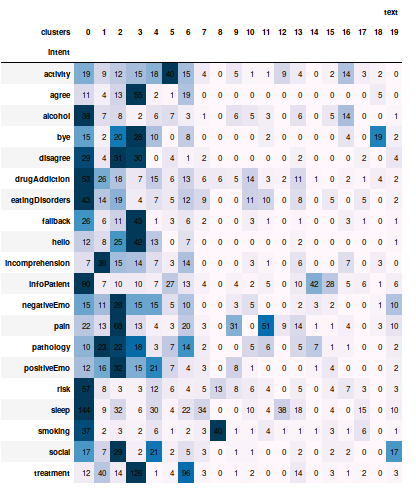
\includegraphics[scale=0.28]{lda_ac_cm.png}
	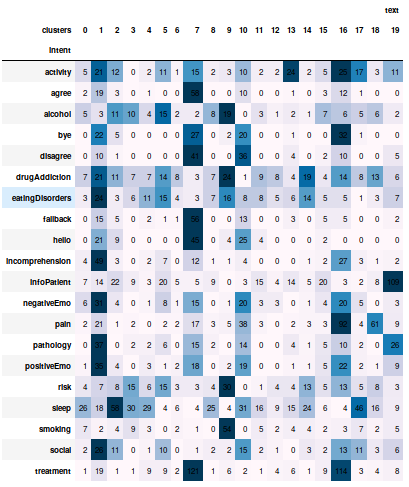
\includegraphics[scale=0.28]{lda_gm_cm.png}
	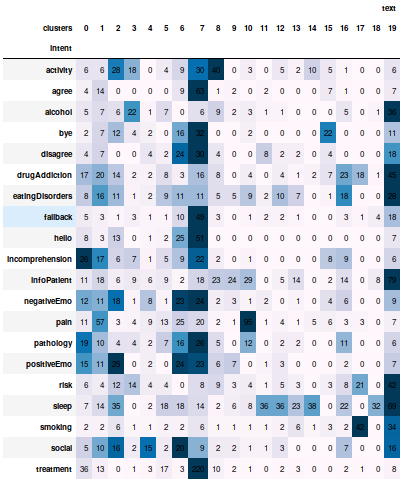
\includegraphics[scale=0.28]{lda_km_cm.png}
	\caption{LDA confusion matrixes: agglomerative clustering, gaussian mixture, Kmeans}
\label{lda_gm_cm}
\end{figure}
\FloatBarrier

Thanks to confusion matrix that is constructed based on cluster and
intent labels we can make hypotheses about possible errors and
difficulties and figure out what connections our model distinguishes
well. Though different clustering algorithms still capture different
connections between intents, there are some common errors for all of
them. In particular, the following intent are incorrectly clustered
together: fallback and hello; alcohol, drugAddiction and risk; social
and emotions.

%\subsubsection{GloVe pretrained}
\subsubsection{Google News W2V pretrained}
We used word2vec google-news model with 300 dimensional feature space.
CV 0.418 + 0.057%
\subsubsection{CNN by word}
From simple encoder, w2v, lda, w2v + lda

\subsubsection{BiLSTM by word}

Following ( et al.) we trained BiLSTM encoder model verifying the best params. So we iterated through the number of layres, it's dimention and type of pooling.

\begin{table}[htb]
\begin{center}
\begin{tabular}{ |r|c|c|c|c|c| }
\hline
layers & purity  & silhouette  & homogeneity  & completeness \\ \hline 
1  & \textbf{0.286369}  & 0.239979  & \textbf{0.227069}  & \textbf{0.232338}\\ \hline 
2  & 0.262836  & 0.181804  & 0.211068  & 0.219279\\ \hline 
3  & 0.238284  & 0.266460  & 0.195002  & 0.206703\\ \hline 
4  & 0.218623  & \textbf{0.439161}  & 0.164478  & 0.192599
\end{tabular}
\end{center}
\caption{Comparison of models with different number of layers}
\end{table}
\FloatBarrier

So it's better to stay with one layer. Now for one layer we test its dimension.

\begin{table}[htb]
\begin{center}
\begin{tabular}{ |r|c|c|c|c|c| }
\hline
layers & purity  & silhouette  & homogeneity  & completeness \\ \hline 
32  & 0.270273  & 0.244798  & 0.214607  & 0.21474\\ \hline 
64  & \textbf{0.281683}  & 0.22728  & 0.231666  & 0.232176\\ \hline 
128  & 0.271597  & 0.263519  & \textbf{0.234111}  & \textbf{0.235486}\\ \hline 
256  & 0.270681  & 0.267634  & 0.229275  & 0.231675\\ \hline 
512  & 0.277608  & 0.264844  & 0.231268  & 0.235075\\ \hline 
1024  & 0.266707  & 0.260425  & 0.226291  & 0.229238\\ \hline 
2048  & 0.268796  & \textbf{0.278391}  & 0.228211  & 0.231041 \\ \hline
\end{tabular}
\end{center}
\caption{Dimension choosing}
\end{table}
\FloatBarrier

Finally, we chose 64 output size due to bigger difference in purity score.

Next step is chose what encoder should we use: last hiiden layer or mean-pooling or max pool on them?

\begin{table}[htb]
\begin{center}
\begin{tabular}{ |r|c|c|c|c|c| }
\hline
last layer & purity  & silhouette  & homogeneity  & completeness \\ \hline 
last hidden & 0.281683  & 0.22728  & 0.231666  & 0.232176\\ \hline 
mean hidden & 0.255399 &	0.170045 	& 0.194848 	& 0.196056 \\ \hline
max hidden  &	0.272616 	& 0.177766 	& 0.218339 	& 0.219109 \\ \hline
\end{tabular}
\end{center}
\caption{Choosing pooling}
\end{table}
\FloatBarrier

Finally we got BiLSTM model with one 64-dimensional layer without pooling.

\begin{figure}[h]
	\centering
	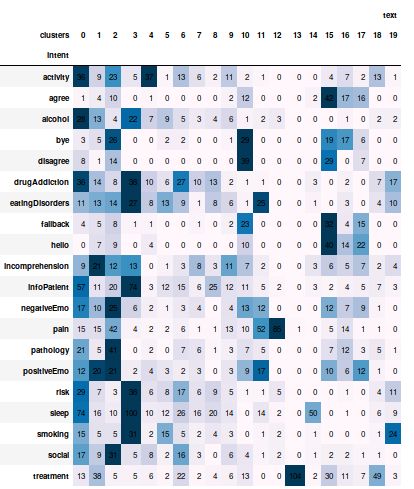
\includegraphics[scale=0.28]{bilstm_ac_cm.png}
	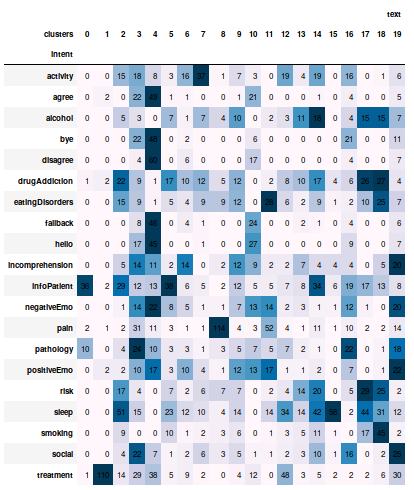
\includegraphics[scale=0.28]{bilstm_gm_cm.png}
	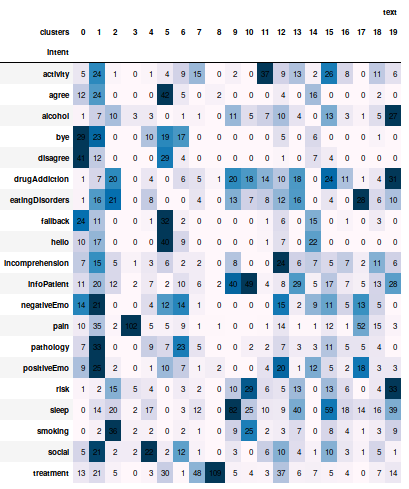
\includegraphics[scale=0.28]{bilstm_km_cm.png}
	\caption{BiLSTM confusion matrixes: : agglomerative clustering, gaussian mixture, Kmeans}
\label{lda_gm_cm}
\end{figure}
\FloatBarrier

This model shows really good separatation for treatment and pain labels, 
tends to group together (agree, fallback and hello) and (bye and disagree).

\subsubsection{Overall comparison}



\begin{table}[htb]
\begin{center}
\begin{tabular}{ |r|c|c|c|c|c| }
\hline
model & features & purity  & silhouette  & homogeneity  & completeness \\ \hline 
W2V 	& 10   & 0.192032  & 0.077404  & 0.108761  & 0.127672 \\ \hline 
W2V 	& 100  & 0.184266  & 0.065381  & 0.109944  & 0.144074 \\ \hline 
LDA 	& 400  & 0.272718  & 0.192777  & 0.177547  & 0.192270 \\ \hline 
BiLSTM 	& 64  & \textbf{0.281683}  & 0.22728  & 0.231666  & 0.232176\\ \hline 
\end{tabular}
\end{center}
\caption{Overall comparison}
\end{table}
\FloatBarrier



\subsection{Classifier}
\label{subsec:classifying2}
\add{training on labelled data (cf. Section \ref{subsec:labelleddata})}

\subsubsection{Evaluation metrics}

A classical way to evaluate a classification model performance is using accuracy score. Sometimes, especially in case of unbalanced dataset, it can be misleading because it can represent that model learns just one class. It’s better to look for a precision score as a measure of exactness and a recall score as a measure of completeness.

\begin{equation}
P = \frac{TP}{TP+FP} 
\end{equation}

\begin{equation}
R = \frac{TP}{TP+FN}
\end{equation}

where TP - True Positives, FP - False Positives, FN - False Negatives.

If we want to get an idea how our classifier deals with both classes (in simple binary case) we should use F1 score that conveys the balance between the precision and the recall.
\begin{equation}
F1 = \frac{2*P*R}{P+R}
\end{equation}

    There is a more clean and unambiguous way to describe the model behaviour that is a confusion matrix. The bigger values on the main diagonal the better as well as the more balanced small values on antidiagonal.

\begin{table}[htb]
\begin{center}
\begin{tabular}{ |r|c|c| }
\hline
& Real positive & Real negative \\ \hline
Predicted positive & True Positive 	& False Positive \\ \hline
Predicted negative & False negative & True negative \\ \hline
\end{tabular}
\caption{Confusion matrix template}
\end{center}
\end{table}
\FloatBarrier

\subsubsection{Results}

For training train and test dataset were created with 65 and 43 items respectively that makes 60/40 ratio. Both are balanced \add{each category has the same number of items}. 

SVC model was chosen with the best parameters by using Grid Search. We are comparing two kernels - rbf (C=10, gamma=1) and linear (C=10, gamma=0.001). For each model, we use 5 fold cross validation.
5-folds Cross Validation error on train set 0.401 + 0.0115 and on test set 0.371 + 0.0338. Small %difference in score indicates good performance and absence of overfitting. 

\begin{table}[htb]
\begin{center}
\begin{tabular}{ |p{2cm}|c|c|c|c|c| }
\hline
Kernel 	& Train & Test & precision & recall & F1 \\ \hline
rbf		& 0.524 + 0.00717 & 0.387 + 0.0341 & 0.308 & 0.316 & 0.287 \\ \hline
linear	& 0.371 + 0.00787 & 0.338 + 0.0431 & 0.238 & 0.241 & 0.215 \\ \hline
\end{tabular}
\caption{CV score comparison}
\end{center}
\end{table}
\FloatBarrier

Though model with rbf model has higher scores, the linear one is less prone to overfitting as shown by the small difference between train and test errors. It was decided to try both and observe their behavior.

\begin{figure}[h]
	\centering
	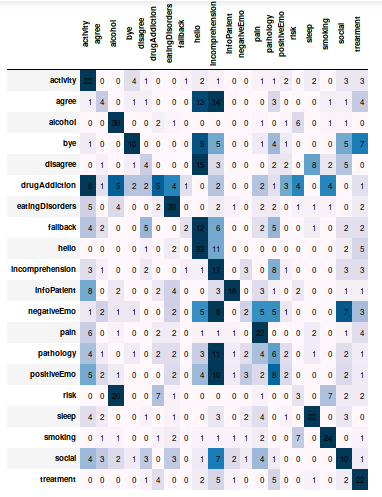
\includegraphics[scale=0.40]{svc0_cm.png}
	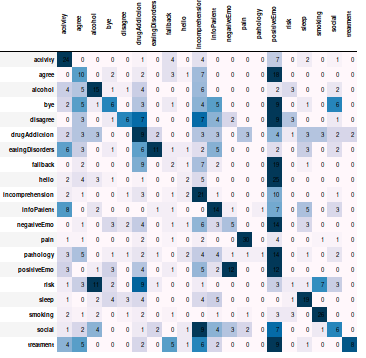
\includegraphics[scale=0.40]{lsvc_0.png}
	\caption{SVC confusion matrix}
\label{lda_gm_cm}
\end{figure}
\FloatBarrier


\subsection{Semi Supervised Learning with linear kernel}
\label{subsec:semisupervised}
\add{now give classifier results obtained after each data expansion step (cf. \ref{subsec:dataexpansion}}.
  
\paragraph{Iteration 0 (Baseline).} 

\add{no data expansion; trained on gold data}

\begin{table}[htb]
\begin{center}
\begin{tabular}{ |r|c|c|c|c|c|c| }
\hline
label & precision    & recall  & f1-score   & support\\ \hline 
\\ \hline 
activity &  0.56 & 0.36 & 0.44 &   66\\ \hline 
agree &  0.23 & 0.19 & 0.21 &   54\\ \hline 
alcohol &  0.35 & 0.34 & 0.34 &   44\\ \hline 
bye &  0.14 & 0.24 & 0.18 &   25\\ \hline 
disagree &  0.14 & 0.40 & 0.21 &   15\\ \hline 
drugAddiction &  0.21 & 0.12 & 0.15 &   75\\ \hline 
eatingDisorders &  0.26 & 0.61 & 0.36 &   18\\ \hline 
fallback &  0.05 & 0.09 & 0.06 &   22\\ \hline 
hello &  0.05 & 0.17 & 0.07 &   12\\ \hline 
incomprehension &  0.49 & 0.20 & 0.29 &  103\\ \hline 
infoPatient &  0.33 & 0.25 & 0.29 &   55\\ \hline 
negativeEmo &  0.12 & 0.21 & 0.15 &   24\\ \hline 
pain &  0.70 & 0.81 & 0.75 &   37\\ \hline 
pathology &  0.02 & 0.50 & 0.04 &    2\\ \hline 
positiveEmo &  0.28 & 0.07 & 0.11 &  178\\ \hline 
risk &  0.02 & 0.08 & 0.04 &   12\\ \hline 
sleep &  0.44 & 0.47 & 0.46 &   40\\ \hline 
smoking &  0.60 & 0.68 & 0.64 &   38\\ \hline 
social &  0.14 & 0.20 & 0.16 &   30\\ \hline 
treatment &  0.19 & 0.80 & 0.30 &   10\\ \hline 
\\ \hline 
micro avg &  0.27 & 0.27 & 0.27 &  860\\ \hline 
macro avg &  0.27 & 0.34 & 0.26 &  860\\ \hline 
weighted avg &  0.33 & 0.27 & 0.27 &  860\\ \hline 
\end{tabular}
\caption{Classifier 0}
\end{center}
\end{table}
\FloatBarrier

\paragraph{Iteration 1} For the first iteration we created subset of external data with $N=500$ sentences for each predicted intent, then splitted data into 200 clusters, majority threshold=, hreshold for probability was chosen pretty low(0.12) in order to be able to extend all 20 categories. In result, we achived 15 new items.

\begin{table}[htb]
\begin{center}
\begin{tabular}{ |r|c|c|c|c|c|c| }
label & precision    recall  f1-score   support\\ \hline 
\\ \hline 
activity &  0.30 & 0.27 & 0.28 &   49\\ \hline 
agree &  0.16 & 0.28 & 0.21 &   25\\ \hline 
alcohol &  0.53 & 0.44 & 0.48 &   52\\ \hline 
bye &  0.33 & 0.41 & 0.36 &   34\\ \hline 
disagree &  0.14 & 0.08 & 0.10 &   78\\ \hline 
drugAddiction &  0.21 & 0.29 & 0.24 &   31\\ \hline 
eatingDisorders &  0.37 & 0.73 & 0.49 &   22\\ \hline 
fallback &  0.12 & 0.31 & 0.17 &   16\\ \hline 
hello &  0.00 & 0.00 & 0.00 &   19\\ \hline 
incomprehension &  0.37 & 0.26 & 0.31 &   61\\ \hline 
infoPatient &  0.49 & 0.34 & 0.40 &   61\\ \hline 
negativeEmo &  0.05 & 0.06 & 0.05 &   31\\ \hline 
pain &  0.60 & 0.46 & 0.53 &   56\\ \hline 
pathology &  0.05 & 0.09 & 0.06 &   23\\ \hline 
positiveEmo &  0.37 & 0.11 & 0.17 &  142\\ \hline 
risk &  0.12 & 0.16 & 0.13 &   32\\ \hline 
sleep &  0.42 & 0.50 & 0.46 &   36\\ \hline 
smoking &  0.44 & 0.59 & 0.51 &   32\\ \hline 
social &  0.14 & 0.21 & 0.17 &   28\\ \hline 
treatment &  0.58 & 0.78 & 0.67 &   32\\ \hline 
\\ \hline 
micro avg &  0.29 & 0.29 & 0.29 &  860\\ \hline 
macro avg &  0.29 & 0.32 & 0.29 &  860\\ \hline 
weighted avg &  0.33 & 0.29 & 0.29 &  860\\ \hline
\end{tabular}
\caption{Classifier 1}
\end{center}
\end{table}
\FloatBarrier

\paragraph{Iteration 2} For the second iteration we created subset of external data with $N=200$ sentences for each predicted intent, then splitted data into 200 clusters, majoiry threshold=, hreshold for probability was chosen pretty low(0.1) in order to be able to extend all 20 categories. In result, we achived 13 new items.

\begin{table}[htb]
\begin{center}
\begin{tabular}{ |r|c|c|c|c|c|c| }
label  &    precision    recall  f1-score   support\\ \hline 
\\ \hline 
activity &  0.42 & 0.29 & 0.34 &   63\\ \hline 
agree &  0.05 & 0.12 & 0.07 &   17\\ \hline 
alcohol &  0.56 & 0.49 & 0.52 &   49\\ \hline 
bye &  0.53 & 0.38 & 0.44 &   61\\ \hline 
disagree &  0.37 & 0.38 & 0.38 &   42\\ \hline 
drugAddiction &  0.23 & 0.23 & 0.23 &   43\\ \hline 
eatingDisorders &  0.28 & 0.34 & 0.31 &   35\\ \hline 
fallback &  0.00 & 0.00 & 0.00 &    6\\ \hline 
hello &  0.21 & 0.43 & 0.28 &   21\\ \hline 
incomprehension &  0.35 & 0.20 & 0.25 &   76\\ \hline 
infoPatient &  0.49 & 0.44 & 0.46 &   48\\ \hline 
negativeEmo &  0.16 & 0.21 & 0.18 &   34\\ \hline 
pain &  0.70 & 0.81 & 0.75 &   37\\ \hline 
pathology &  0.05 & 0.29 & 0.08 &    7\\ \hline 
positiveEmo &  0.09 & 0.14 & 0.11 &   29\\ \hline 
risk &  0.07 & 0.11 & 0.08 &   28\\ \hline 
sleep &  0.49 & 0.54 & 0.51 &   39\\ \hline 
smoking &  0.49 & 0.66 & 0.56 &   32\\ \hline 
social &  0.26 & 0.31 & 0.28 &   36\\ \hline 
treatment &  0.56 & 0.15 & 0.24 &  157\\ \hline 
\\ \hline 
micro avg &  0.32 & 0.32 & 0.32 &  860\\ \hline 
macro avg &  0.32 & 0.32 & 0.30 &  860\\ \hline 
weighted avg &  0.40 & 0.32 & 0.33 &  860\\ \hline 
\end{tabular}
\caption{Classifier 1}
\end{center}
\end{table}
\FloatBarrier


\begin{table}[htb]
\begin{center}
\begin{tabular}{ |r|c|c|c|c|c|c| }
\hline
Iteration 	& Score  & CV mean & CV std & precision & recall & F1 \\ \hline
0			& 0.2651 & 0.337   & 0.0503 & 0.265 	& 0.340  & 0.262 \\ \hline
1			& 0.2895 & 0.323   & 0.0212 & 0.289 	& 0.319  & 0.290 \\ \hline
2 			& 0.3174 & 0.333   & 0.0118 & 0.317 	& 0.325  & 0.304 \\ \hline
\end{tabular}
\caption{Classifier scores comparison}
\end{center}
\end{table}
\FloatBarrier

\begin{figure}[h]
	\centering
	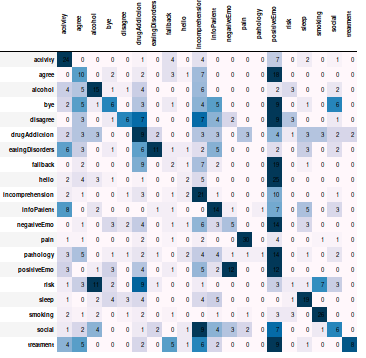
\includegraphics[scale=0.3]{lsvc_0.png}
	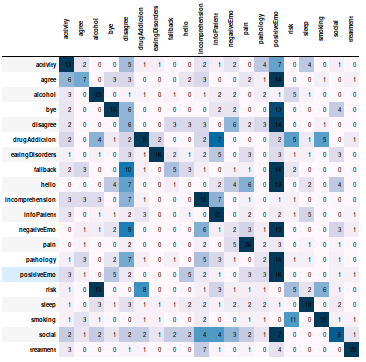
\includegraphics[scale=0.3]{lsvc_1.png}
	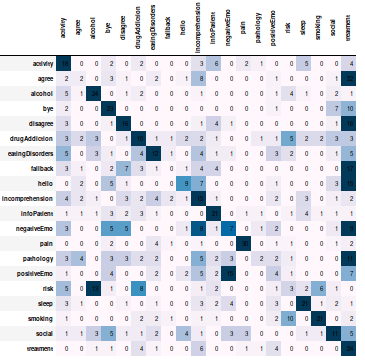
\includegraphics[scale=0.3]{lsvc_2.png}
	\caption{SVC confusion matrix}
\label{lda_gm_cm}
\end{figure}
\FloatBarrier


\subsection{Semi-supervised learning with rbf kernel}
\label{subsec:semisupervised-rbf}

\paragraph{Iteration 0.}
\begin{table}[htb]
\begin{center}
\begin{tabular}{ |r|c|c|c|c| }
\hline
intent &precision & recall & f1-score & support\\ \hline 
activity & 0.44 & 0.40 & 0.42 &  47\\ \hline 
agree & 0.72 & 0.20 & 0.32 & 152\\ \hline 
alcohol & 0.51 & 0.44 & 0.47 &  50\\ \hline 
bye & 0.35 & 0.29 & 0.32 &  51\\ \hline 
disagree & 0.33 & 0.38 & 0.35 &  37\\ \hline 
drugAddiction & 0.09 & 0.13 & 0.11 &  30\\ \hline 
eatingDisorders & 0.33 & 0.45 & 0.38 &  31\\ \hline 
fallback & 0.00 & 0.00 & 0.00 &   8\\ \hline 
hello & 0.23 & 0.25 & 0.24 &  40\\ \hline 
incomprehension & 0.51 & 0.29 & 0.37 &  76\\ \hline 
infoPatient & 0.30 & 0.54 & 0.39 &  24\\ \hline 
negativeEmo & 0.12 & 0.19 & 0.14 &  26\\ \hline 
pain & 0.30 & 0.22 & 0.25 &  59\\ \hline 
pathology & 0.09 & 0.16 & 0.12 &  25\\ \hline 
positiveEmo & 0.09 & 0.17 & 0.12 &  24\\ \hline 
risk & 0.05 & 0.17 & 0.07 &  12\\ \hline 
sleep & 0.42 & 0.58 & 0.49 &  31\\ \hline 
smoking & 0.65 & 0.61 & 0.63 &  46\\ \hline 
social & 0.33 & 0.50 & 0.39 &  28\\ \hline 
treatment & 0.51 & 0.35 & 0.42 &  63\\ \hline 
\\ \hline 
micro avg & 0.32 & 0.32 & 0.32 & 860\\ \hline 
macro avg & 0.32 & 0.32 & 0.30 & 860\\ \hline 
weighted avg & 0.42 & 0.32 & 0.34 & 860\\ \hline 
\end{tabular}
\caption{Intention mean probability}
\end{center}
\end{table}
\FloatBarrier


\paragraph{Iteration 1} For the first iteration we created subset of external data with $N=500$ sentences for each predicted intent, then splitted data into 1000 clusters, majoiry threshold=, hreshold for probability was chosen pretty low(0.15) in order to be able to extend all 20 categories. In result, we achived 6 new items.

\begin{table}[htb]
\begin{center}
\begin{tabular}{ |r|c|c|c|c| }
\hline
label & precision & recall & f1-score &  support\\ \hline 
\\ \hline 
activity &  0.49 & 0.54 & 0.51 &   39\\ \hline 
agree &  0.23 & 0.31 & 0.27 &   32\\ \hline 
alcohol &  0.56 & 0.41 & 0.47 &   59\\ \hline 
bye &  0.28 & 0.67 & 0.39 &   18\\ \hline 
disagree &  0.33 & 0.31 & 0.32 &   45\\ \hline 
drugAddiction &  0.26 & 0.39 & 0.31 &   28\\ \hline 
eatingDisorders &  0.47 & 0.67 & 0.55 &   30\\ \hline 
fallback &  0.26 & 0.12 & 0.17 &   88\\ \hline 
hello &  0.51 & 0.25 & 0.34 &   88\\ \hline 
incomprehension &  0.30 & 0.29 & 0.30 &   45\\ \hline 
infoPatient &  0.42 & 0.35 & 0.38 &   52\\ \hline 
negativeEmo &  0.05 & 0.06 & 0.05 &   36\\ \hline 
pain &  0.65 & 0.49 & 0.56 &   57\\ \hline 
pathology &  0.14 & 0.35 & 0.20 &   17\\ \hline 
positiveEmo &  0.14 & 0.20 & 0.16 &   30\\ \hline 
risk &  0.07 & 0.14 & 0.09 &   21\\ \hline 
sleep &  0.58 & 0.66 & 0.62 &   38\\ \hline 
smoking &  0.51 & 0.54 & 0.52 &   41\\ \hline 
social &  0.19 & 0.29 & 0.23 &   28\\ \hline 
treatment &  0.63 & 0.40 & 0.49 &   68\\ \hline 
\\ \hline 
micro avg &  0.35 & 0.35 & 0.35 &  860\\ \hline 
macro avg &  0.35 & 0.37 & 0.35 &  860\\ \hline 
weighted avg &  0.40 & 0.35 & 0.36 &  860\\ \hline 
\end{tabular}
\caption{Classification report for first iteration}
\end{center}
\end{table}
\FloatBarrier


\begin{figure}[h]
	\centering
	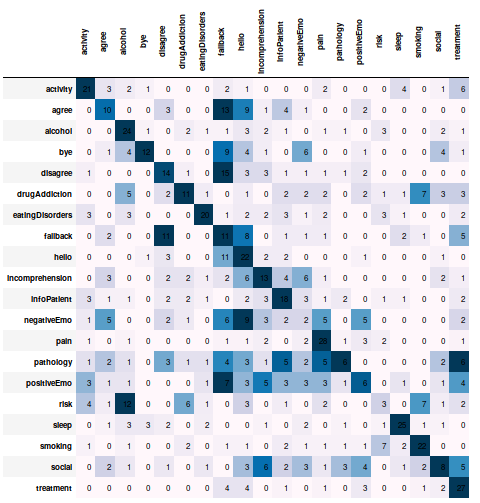
\includegraphics[scale=0.40]{svc1_cm.png}
	\caption{SVC confusion matrix}
\label{lda_gm_cm}
\end{figure}
\FloatBarrier

\paragraph{Iteration 2.} For the first iteration we created subset of external data with $N=500$ sentences for each predicted intent, then splitted data into 1000 clusters, majoiry threshold=, hreshold for probability was chosen pretty low(0.11) in order to be able to extend all 20 categories. In result, we achived 5 new items.

\begin{table}[htb]
\begin{center}
\begin{tabular}{ |r|c|c|c|c| }
\hline
label  &    precision & recall & f1-score  & support\\ \hline 
\\ \hline 
activity 		& 0.37 &   0.34 &   0.36 & 47\\ \hline 
agree 			& 0.14 &   0.21 &   0.17 & 29\\ \hline 
alcohol 		& 0.47 &   0.39 &   0.43 & 51\\ \hline 
bye 			& 0.33 &   0.30 &   0.31 & 46\\ \hline 
disagree 		& 0.35 &   0.43 &   0.38 & 35\\ \hline 
drugAddiction 	& 0.28 &   0.29 &   0.28 & 42\\ \hline 
eatingDisorders & 0.33 &   0.25 &   0.28 & 57\\ \hline 
fallback 		& 0.14 &   0.12 &   0.13 & 51\\ \hline 
hello 			& 0.40 &   0.19 &   0.26 & 90\\ \hline 
incomprehension & 0.42 &   0.43 &   0.42 & 42\\ \hline 
infoPatient 	& 0.37 &   0.52 &   0.43 & 31\\ \hline 
negativeEmo 	& 0.14 &   0.18 &   0.16 & 34\\ \hline 
pain 			& 0.49 &   0.44 &   0.46 & 48\\ \hline 
pathology 		& 0.16 &   0.29 &   0.21 & 24\\ \hline 
positiveEmo 	& 0.16 &   0.20 &   0.18 & 35\\ \hline 
risk 			& 0.05 &   0.11 &   0.06 & 19\\ \hline 
sleep 			& 0.56 &   0.63 &   0.59 & 38\\ \hline 
smoking 		& 0.58 &   0.54 &   0.56 & 46\\ \hline 
social 			& 0.21 &   0.56 &   0.31 & 16\\ \hline 
treatment 		& 0.40 &   0.22 &   0.28 & 79\\ \hline 
\\ \hline 
micro avg &    0.32 &   0.32 &   0.32 &    860\\ \hline 
macro avg &    0.32 &   0.33 &   0.31 &    860\\ \hline 
weighted avg & 0.34 &   0.32 &   0.32 &    860\\ \hline 
\\ \hline 
\end{tabular}
\caption{Classification report for the second iteration}
\end{center}
\end{table}
\FloatBarrier

\begin{figure}[h]
	\centering
	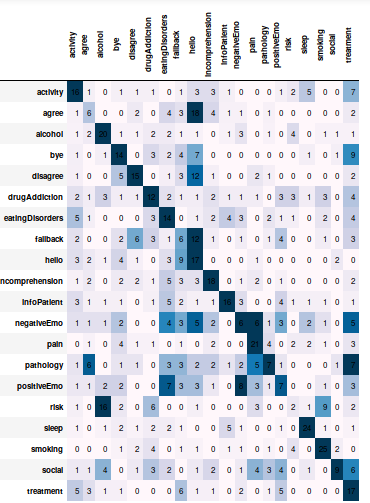
\includegraphics[scale=0.40]{svc2_cm.png}
	\caption{SVC confusion matrix}
\label{lda_gm_cm}
\end{figure}
\FloatBarrier

\paragraph{Overall comparison}

In this section we provide grouped results about classifier scores chaging by iteration. 

\begin{table}[htb]
\begin{center}
\begin{tabular}{ |r|c|c|c|c|c|c| }
\hline
Iteration 	& Score  & CV mean & CV std & precision & recall & F1 \\ \hline
0			& 0.3186 & 0.371   & 0.0338 & 0.308 	& 0.316  & 0.287 \\ \hline
1			& 0.3523 & 0.350   & 0.0153 & 0.352 	& 0.371  & 0.346 \\ \hline
2 			& 0.3167 & 0.332   & 0.0150 & 0.316 	& 0.331  & 0.313 \\ \hline
\end{tabular}
\caption{Classifier scores comparison}
\end{center}
\end{table}
\FloatBarrier

\begin{table}[htb]
\begin{center}
\begin{tabular}{ |r|c|c|c| }
\hline
Intent & It 0 & It 1 & It 2 \\ \hline
activity		& 0.31+0.10 & 0.51+0.02	\\ \hline
agree 			& 0.17+0.06 & 0.32+0.01	\\ \hline
alcohol 		& 0.37+0.13 & 0.53+0.03	\\ \hline
bye 			& 0.17+0.03 & 0.40+0.03	\\ \hline
disagree 		& 0.19+0.03 & 0.27+0.03	\\ \hline
drugAddiction 	& 0.22+0.06 & 0.32+0.03 \\ \hline
eatingDisorders & 0.33+0.13 & 0.66+0.07 \\ \hline
fallback 		& 0.16+0.03 & 0.19+0.05	\\ \hline
hello 			& 0.17+0.02 & 0.31+0.14	\\ \hline
incomprehension & 0.20+0.04 & 0.46+0.02	\\ \hline
infoPatient 	& 0.39+0.18 & 0.71+0.05 \\ \hline
negativeEmo 	& 0.17+0.03 & 0.34+0.06 \\ \hline
pain 			& 0.36+0.14 & 0.67+0.05 \\ \hline
pathology 		& 0.16+0.04 & 0.39+0.06 \\ \hline
positiveEmo 	& 0.19+0.04 & 0.27+0.03 \\ \hline
risk 			& 0.28+0.07 & 0.31+0.03 \\ \hline
sleep 			& 0.42+0.18 & 0.96+0.01 \\ \hline
smoking 		& 0.49+0.17 & 0.79+0.02 \\ \hline
social 			& 0.23+0.07 & 0.38+0.04 \\ \hline
treatment 		& 0.25+0.04 & 0.43+0.04 \\ \hline
\end{tabular}
\caption{Intention mean probability}
\end{center}
\end{table}
\FloatBarrier

\begin{figure}[h]
	\centering
	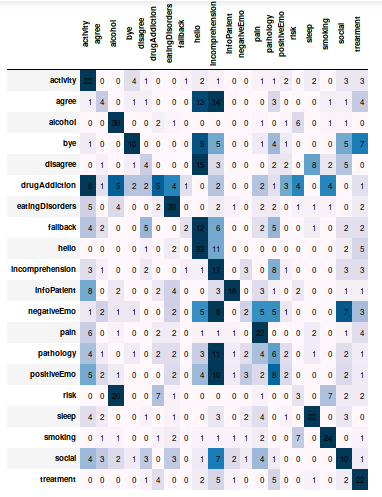
\includegraphics[scale=0.25]{svc0_cm.png}
	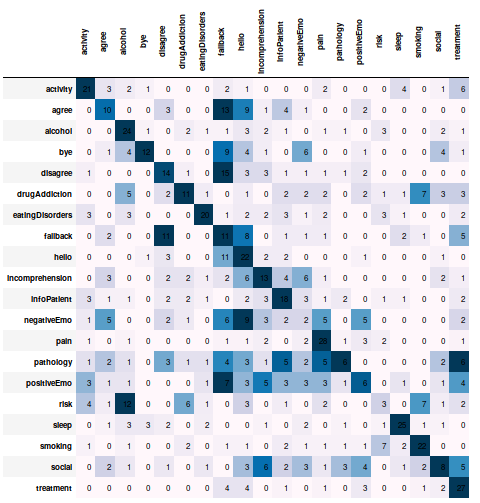
\includegraphics[scale=0.25]{svc1_cm.png}
	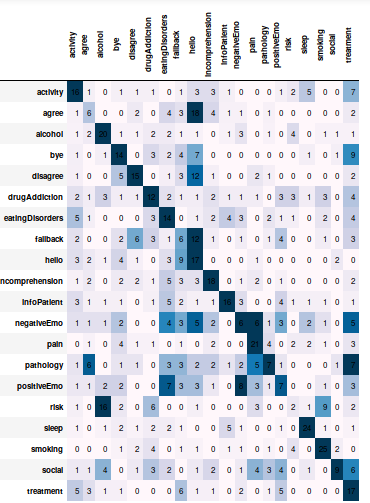
\includegraphics[scale=0.25]{svc2_cm.png}
	\caption{SVC confusion matrix}
\label{lda_gm_cm}
\end{figure}
\FloatBarrier


\section{Conclusion and future work}
\label{sec:conclusion}

In this project we were dealing with task of paraphrase detection for expanding initial dataset. Our approch is to train the word embedding model that will be able to provide clusters similar to initial classes. We used LDA and W2V models for that and later trained SVC and Kmeans models to label external data and chose the representative example to extend existing dataset and retrain models on it.

Our results shows how high rate of confusion between labels in intial classifier increases this confusion in futher data expansion though in general algorithms tends to converge to be more precise. Also, the more data you have the higher chances to find more similar sentences to initial one so that possible context for each intent will grow gradually.

Future work will be devoted to improving word embedding model, trying one-shot learning model in order to improve classification score. Transfering from one-intent to multi-intent is preferable due to the fact that sentences are usually ambiguous than not. Another possible direction for development can be creating framework for adding new labels to the existing classifier.

\section{References}
\bibliographystyle{alpha}
\bibliography{biblio}
$ Ward J.H. Hierarchical grouping to optimize an objective function // J. of the American Statistical Association, 1963. — 236 р. $

\end{document}
